% !TEX root = ../Coherence2.tex

\section{Contextual families of nestohedra} 
\label{s:contextual}

In this section, we define a subclass of the class of  nestohedra, which, as we shall argue, brings us even closer to
our favourite categorical coherence results. We begin by giving some intuition.

\subsection{Discussion} \label{contextual-discussion}

In the previous section, we have established coherence (in our polytopal sense) using standard term rewriting methods. So far so good. But  it can be argued that constructs are more economical than the terms on the signatures that we have introduced, and that, being themselves trees, they ``look like" terms. 
Can we somehow reproduce our discussion of rewriting, and in particular of critical pairs, directly on constructs?

An obstacle is that the bijection $\chi$ of~ \cref{l:bijection-terms} strips off useful information on the support of all subconstructions (i.e.,  subtrees) of the constructions to be ``rewritten''.  Taking~ \cref{l:instantiation-constructions} seriously, one can be tempted to consider $x(y(\cdots),\cdots)< y(x(\cdots),\cdots)$ as a rewrite rule (for $x<y$), but filling in the $\cdots$ requires knowing the support $K$ of $\occ{S}{x}$.  So, at the price of reconstructing $K$ from the inductive definition of $S$,  this description is acceptable. But for the study of critical confluence diagrams, say   $S < x_2(x_1(x_3,\cdots),\cdots),\cdots)$ and $S < x_3(x_1(\cdots),x_2(\cdots),\cdots)$, for $S\eqdef  x_1(x_2(\cdots),x_3(\cdots),\cdots)$, can we be sure that the shape of the local confluence diagram will be independent of the support of $\occ{S}{x_1}$?  

In view of~ \cref{instance-construct-general}, this shape is
$\recrestr{(\hyper{H}_{\supp(\occ{T}{x_1})})}{\set{x_1,x_2,x_3}}$.  It would be more satisfying if the shape was
$\recrestr{\hyper{H}}{\set{x_1,x_2,x_3}}$, because then the critical confluence diagram would be ``context-independent'' (for this informal notion of rewriting), i.e., all $\set{x_1,x_2,x_3}$-faces would have the same shape.
This motivates the definition of contextual hypergraph below. 



%%%%%%%%%%%%%%%%%%%%%%%%%%%%%%%%%%%%%%%

\subsection{Contextual nestohedra}

\begin{definition} 
A connected hypergraph $\hyper{H}$ is \defn{contextual} if, for all connected subsets $Y\inc H$ of cardinal $|Y|\geq 3$, and for all $3$-elements subsets $X=\{x,y,z\} \subseteq Y$, one of the following equivalent conditions is satisfied:
\begin{enumerate}
\item
$\begin{array}{lll}
  \xyz{x}{{\hyper{H}_Y}}{\set{y,z}} & \Leftrightarrow & \xyz{x}{\hyper{H}}{\set{y,z}}
  \end{array}$,
\item
$\hyper{H}_{\cap X} = (\hyper{H}_Y)_{\cap X}$.
\end{enumerate}
\end{definition}
That these conditions are equivalent   is a direct consequence of~\cref{xyz-reconnected}.
We first give two examples of hypergraphs that are \emph{not} contextual.
%We start with two motivating counter-examples (in reference to the discussion above).

%Now, if $T'$ is another $X$-face and $\occ{T'}{X}\neq T'$, then we would like to see  $T'$ as $\occ{T'}{X}$ in context, and hence $T'$ as ``$X$ in situation''.  
%For this to hold, $T'$ should be of the same form as $T$. 
%Setting $Y\eqdef \supp(\occ{T}{X})$, we have that the poset of faces of $T'$ is isomorphic to the poset of faces of $\occ{T'}{X}$, which is a construct of $\hyper{H}_Y$ and has $X$ as root, so is in turn isomorphic to the poset of faces of $\recrestr{\hyper{(\hyper{H}_Y)}}{X}$ (\cref{instance-construct}).
%Is it always the case that $\recrestr{(\hyper{H}_Y)}{X}=\recrestr{\hyper{H}}{X}$ for~$Y$ connected in $\hyper{H}$? 
%The following examples give a negative answer.

\begin{example} 
  \label{non-contextual-1}
Consider the hypergraph 
\[
  \hyper{H}\eqdef  \set{\set{x},\set{y},\set{z},\set{u},\set{x,y,z}, \set{x,u,z}},
  \]
the set $X\eqdef \set{x,y,z}$ and the two $X$-faces $S\eqdef u(X)$ and $T\eqdef X(u)$. 
Then $\occ{S}{X}$ is a construct of $\hyper{K}\eqdef \restrH{H}{\set{u}}$ while $\occ{T}{X}=T$ is a construct of $\hyper{H}$.
But we have $\xyz{y}{\hyper{K}}{\set{x}\!,\!\set{z}}$ and $\xyz{y}{\hyper{H}}{\set{x,z}}$, which implies that $S$ is a triangle while $T$ is a quadrilateral, as
$\recrestr{\hyper{K}}{\set{x,y,z}} = \hyper{K}  =  \set{\set{x},\set{y},\set{z},\set{x,y,z}}$ and $\recrestr{\hyper{H}}{\set{x,y,z}}  =  \set{\set{x},\set{y},\set{z},\set{u},\set{x,z}\set{x,y,z}}$. Therefore $\hyper{H}$ is not contextual.
\end{example}
  
\begin{example} 
  \label{non-contextual-2}
Consider the graph 
$$\set{\set{x},\set{y},\set{z},\set{u},\set{x,y}, \set{y,z}, \set{x,u}, \set{u,z}}.$$
Then exactly the same data as in~ \cref{non-contextual-1} provide evidence that this graph, whose realization is the three-dimensional cyclohedron, is not contextual. 
\end{example}

%This motivates the following definition.

The following Proposition allows us to see all $X$-faces as ``instantiations in context'' of~$\recrestr{\hyper{H}}{X}$.

\begin{proposition} \label{situation-construct}
Let $\hyper{H}$ be a contextual hypergraph.
If $X$ is a subset of $H$ such that $|X|=3$ and $T$ is an $X$-face of $\hyper{H}$, then the poset of faces of $T$ is isomorphic to the poset of faces of~$\recrestr{\hyper{H}}{X}$.
\end{proposition}

\begin{proof}  This is a direct consequence of~ \cref{instance-construct-general}.
%  Let $\hyper{K}\eqdef \hyper{H}_{\supp(S)}$ where $S\eqdef \occ{T}{X}$. 
%  By \cref{subconstruct-restriction}, $S$ is a constuct of $\hyper{K}$. By definition of the face relation, and since the only non-singleton (and hence ``splittable'') node of $T$ is $X$, we have that the poset of subfaces of $T$ is isomorphic to the poset of subfaces of $S$, which by \Cref{instance-construct} is isomorphic to ${\cal A}(\recrestr{\hyper{K}}{X})$, which is isomorphic to ${\cal A}(\recrestr{\hyper{H}}{X})$ since~$\hyper{H}$ is contextual.
\end{proof}




%%%%%%%%%%%%%%%%%%%%%%%%%%%%%%%%%%%%%%%%%%%%%%%%%%%%%%%

\subsection{Contextual families}

Motivated by the examples presented in \cref{ss:hypergraph-polytopes}
% ss:examples} 
and their associated categorical coherence theorems listed in \cref{table:contextual-hyper}, we define now the notion of a contextual \emph{family} of nestohedra.

Identifying a hypergraph $\hyper{H}$ with the maximal construct $T$ of $({\cal A}(\hyper{H}),\preceq)$, we say that $\hyper{H}$ has \defn{dimension} $\dim T$ (cf.  \cref{two-types}).
For a family of hypergraphs $\calH$, we denote by $\calH(n)$ the subset of hypergraphs of dimension $n \geq 0$.

We will consider families of ordered hypergraphs. 
Note that when $\hyper{H}$ is ordered, all the restrictions $\hyper{H}_X$ and reconnected restrictions $\hyper{H}_{\cap X}$ are naturally ordered hypergraphs.

\begin{definition}
  \label{def:contextual-family}
    A family $\calH$ of ordered hypergraphs is \defn{contextual} if 
    \begin{enumerate}
      \item any ordered hypergraph $\hyper{H} \in \calH$ is contextual,
      \item for any $\hyper{H} \in \calH$ and any $X \subseteq H$, all the connected components of $\hyper{H}\setminus X$ are in $\calH$,
      \item we have $\{\hyper{H}_{\cap X} \ | \ X \subset H, |X|=3, \hyper{H} \in \calH \} \subseteq \calH(2)$.
    \end{enumerate}
\end{definition}
As for point (3) of this definition, we note that a reconnected restriction of a contextual hypergraph is contextual.

The term rewriting systems from \cref{ss:rewriting-constructs,ss:rewriting-constructions} can be adapted to a rewriting system on \emph{all} hypergraphs of $\calH$.
We shall focus on the constructions rewriting system. 

\begin{definition}
  For a contextual family of hypergraphs $\calH$, we consider the \defn{constructions signature}~$\Sigma_\calH^c$ defined by the following data:
  \begin{itemize}
    \item Variables and sorts are elements of $\calH$.
    \item Function symbols are pairs of a hypergraph $\hyper{H} \in \calH$ and one of its vertices:
    $$F\eqdef \{(x,\hyper{H}) \ | \ x \in H, \ \hyper{H} \in \calH \}.$$
    \item For $(x,\hyper{H}) \in F$, we define $\ari(x,\hyper{H})$ as the number of connected components of~$\hyper{H} \setminus {x}$.
    \item Variables $\hyper{H} \in V$ are their own sort $\outsort(\hyper{H})\eqdef \hyper{H}$, while function symbols~$(x,\hyper{H}) \in F$ are of sort $\outsort(x,\hyper{H})\eqdef \hyper{H}$.
    \item For function symbols $(x,\hyper{H}) \in F$ such that $\hyper{H},x \leadsto H_1,\ldots,H_n$, and for $1 \leq i \leq n$, we define $\insort((x,\hyper{H}),i)\eqdef \hyper{H}_i$.
  \end{itemize}
\end{definition}

It follows from~\cref{def:contextual-family} and the fact that the restriction of a contextual hypergraph is contextual, that this signature is well-defined.
Moreover, it is straightforward to adapt \cref{l:bijection-constructions} and \cref{def:rules-2} to obtain a term rewriting system $(\Sigma_\calH,R_\calH)$ on the constructions of $\calH$. 

From \cref{thm:critical-pairs}, we have that all local confluence diagrams for overlapping pairs $(\Sigma_\calH,R_\calH)$ correspond to some $X$-face of some $\hyper{H} \in \calH$.
% for $X \subseteq H$, $|X|=3$ and . 
The fact that $\calH$ is contextual imposes an additional uniformity constraint on these diagrams.

\begin{thm}
Let $\calH$ be a contextual family of ordered hypergraphs.
For any $\hyper{H} \in \calH$ and subset $X \subseteq H$ with $|X|=3$, all the $X$-faces and hence their associated  overlapping local confluence diagrams 
have the same shape $\hyper{H}_{\cap X}$. 
\end{thm}

\begin{proof} 
This is a direct consequence of~\cref{situation-construct}.
 % The proof is an easy consequence of~\cref{instance-construct} and \cref{situation-construct}. 
\end{proof}

Mimicking~\cref{thm:confluent}, we get that $(\Sigma_\calH,R_\calH)$ is confluent and terminating.
Moreover, in virtue of Condition (3) in \cref{def:contextual-family}, all the critical confluence diagrams of $(\Sigma_\calH,R_\calH)$ are in~$\calH(2)$.
We argue that these diagrams should be called \emph{coherence conditions}, in view of \cref{rem:coherence} as well as the following examples of contextual families and their coherence theorems. 

%%%%%%%%%%%%%%%%%%%%%%%%%%%%%%%%%%%%%%%

\subsection{Examples}
\label{ss:examples}

We call \defn{contextual graph-associahedra} (resp.\ \defn{contextual nestohedra}) the hypergraph polytopes whose underlying hypergraph is a contextual (hyper)graph.
Here, we include a copy of each (hyper)graph for each possible total order on its vertices.
Recall that simplices, cubes, associahedra, permutahedra and operahedra were introduced in \cref{ss:hypergraph-polytopes}.

\begin{samepage}
  \begin{thm}
    \label{thm:examples}
    The following families of hypergraph polytopes are contextual:
    \begin{enumerate}[label=(\alph*)]
      \item simplices,
      \item cubes,
      \item associahedra,
      \item permutahedra,
      \item operahedra,
      \item contextual graph-associahedra,
      \item contextual nestohedra.
    \end{enumerate}
  \end{thm}
\end{samepage}

\begin{proof}
  Let us proceed one family at a time.
  For each one, we check Conditions (1)-(3) in \cref{def:contextual-family}.
  We consider sets of vertices to be $H=\{1,\ldots,n\}$.
  \begin{enumerate}[label=(\alph*)]
    \item Conditions (1)-(3) follow easily from the fact that hyperedges of simplices are all either singletons or the maximal hyperedge.
    \item We first prove Condition (1). 
    Note $\hyper{C}_n$ is saturated, and that $(\hyper{C}_n)_{\set{1,\ldots,m}}=\hyper{C}_m$ if $m\leq n$.
    So we have to check that for all $m\leq n$ and all $i,j,k\leq m$, we have $\xyz{k}{{\hyper{C}_n}}{\set{i,j}}$ iff
    $\xyz{k}{{\hyper{C}_m}}{\set{i,j}}$, which follows immediately from the observation that for all $p\geq m$ we have
    $\xyz{k}{{\hyper{C}_p}}{\set{i,j}}$ iff $i<k$ and $j<k$.
    For Conditions (2) and (3), it suffices to observe that the connected components of $\hyper{C}_n\setminus X$, for some $X$, are all cubes $\hyper{C}_m$ with $m<n$, and that reconnected restrictions of cubes are cubes.
    \item[(c)-(e)] Conditions (1) and (2) follow from the fact that any connected subgraph of a linear (resp. complete, clawfree block) graph is a linear (resp. complete, clawfree block) graph. 
    Condition (3) follows from the fact that any reconnected complement of a subset in a linear (resp. complete, clawfree block) graph is a linear (resp. complete, clawfree block) graph.
    %As to Condition (1), it is proved in~\cite[Lem.~12]{COI} that the connected subsets of $\hyper{L}({\cal T})$ are in bijective correspondence with the subtrees of $\cal T$ having at least two nodes, through a map $E\mapsto  {\cal T}_E$ such that $\hyper{L}({\cal T})_E=\hyper{L}({\cal T_E})$. Suppose, say, that $\set{x,y,z}\inc E$ and $\xyz{x}{\hyper{L}({\cal T})_E}{\set{y},\set{z}}$. Then it means on the tree side that after removing the edge $x$ from ${\cal T}_E$, resulting in two disjoint subtrees ${\cal T}_E^1$ and ${\cal T}_E^2$ of ${\cal T}_E$, we have, say, $y\in{\cal T}_E^1$ and $z\in{\cal T}_E^2$. 
    %On the other hand, removing $x$ from ${\cal T}$ results in subtrees ${\cal T}^1$ and ${\cal T}^2$, containing ${\cal T}_E^1$ and ${\cal T}_E^2$, respectively. 
    %Therefore $\xyz{x}{\hyper{L}({\cal T}))}{\set{y},\set{z}}$. 
    %And vice-versa.
    \item[(f)-(g)] This is immediate from the definitions.
  \end{enumerate}
\end{proof}

%toute restriction d'un hypergraphe contextuel est contextuelle

\begin{rem}
  Note that contextual (hyper)graphs do not contain all graph-associahedra.
  For instance, we have seen in \cref{non-contextual-2} that the cyclohedra are not contextual. 
  It would be interesting to characterize combinatorially contextual (hyper)graphs.
\end{rem}


%%%%%%%%%%%%%%%%%%%%%%%%%%%%%%%%%%%%

\subsection{Categorical coherence}
\label{ss:coherence}

In this final Section, we recall the categorical coherence theorems associated with associahedra and operahedra, and conjecture one for permutahedra.

%%%%%%%%%%%%%%%%%%%%%%%%%%%%%%%%%%%%

\subsubsection{Associahedra}
Recall that the scene is the data of a category $\mathbf C$, a bifunctor $\otimes:\mathbf{C}^2\rightarrow \mathbf C$ and a natural iso $\alpha$ from the functor
$(X,Y,Z)\mapsto (X\otimes Y)\otimes Z$ to the functor  $(X,Y,Z)\mapsto X \otimes (Y\otimes Z)$. 
Mac Lane's coherence theorem states that for any two functors $F,G$ from $\mathbf{C}^{n+1}$ to $\mathbf{C}$ arising from $n$ iterations of $\otimes$, any two  natural transformations $\lambda_1,\lambda_2$ from $F$ to $G$  ``written using $\alpha$ or its inverse'' are equal, provided the statement holds in the following special case, called  {\em coherence condition}: 
\begin{itemize}
\item $F\eqdef (X,Y,Z,U)\mapsto ((X\otimes Y)\otimes Z)\otimes U,$ and $G\eqdef (X,Y,Z,U)\mapsto X\otimes (Y\otimes (Z\otimes U)),$ 
\item $\lambda_1\eqdef (X\otimes\alpha_{Y,Z,U})\circ\alpha_{X,Y\otimes Z,U} \circ (\alpha_{X,Y,Z}\otimes U),$ and $\lambda_2\eqdef  \alpha_{X,Y,Z\otimes U}\circ \alpha_{X\otimes Y,Z,U},$ 
\end{itemize}
i.e. provided the following diagram (Mac Lane's pentagon) commutes:
\begin{center}
\vspace{-.5cm}
$$
 \xymatrix @-1.65pc {&& ((X\otimes Y)\otimes Z)\otimes U \ar @{->}[ddll]^{\alpha_{X,Y,Z}\otimes U} \ar @{->}[dddrr]^{\alpha_{X\otimes Y,Z,U}}&& \\
 &&&&\\
 (X\otimes (Y\otimes Z))\otimes U  \ar @{->}[dd]^{\alpha_{X,Y\otimes Z,U} }&&   && \\
 &&&&(X\otimes Y)\otimes (Z\otimes U) \ar @{->}[dddll]_{\alpha_{X,Y,Z\otimes U}}\\
 X\otimes ((Y\otimes Z)\otimes U) \ar @{->}[ddrr]_{X\otimes\alpha_{Y,Z,U}} &  &\\
 &&&&\\
 &&X\otimes (Y\otimes (Z\otimes U))&&}
$$
\end{center}

Via Huet's correspondence \cite{Huet-notes-cat}, the annotated proof of confluence of the rewriting system $(\Sigma_\calH, R_\calH)$ associated to the contextual family of associahedra $\calH$ provides a proof of Mac Lane's coherence theorem, with the pentagon in $\calH(2)$ acting as the coherence condition. 
The following examples explain the translation between the language of hypergraph polytopes and the language of monoidal categories. 

\begin{example}
Consider the linear tree
\vspace{-.7cm}
\begin{center}
$$\xymatrix @-1.65pc {{\cal T} & \eqdef  &X \ar @{-}[rr]^{1}&& Y \ar @{-}[rr]^{2}&& Z \ar @{-}[rr]^{3}&& U}
  $$
\end{center}
%\vspace{-.2cm}
Then $\hyper{L}({\cal T})$ is the associahedron $\hyper{K}^3$. 
The constructs of ${\cal T}$ decorate a pentagon as follows

\begin{center}
$$\xymatrix @-1.65pc {&& 3(2(1)) \ar @{->}[ddll]_{3(\set{1,2})} \ar @{->}[dddrr]^{\set{2,3}(1)}&& \\
 &&&&\\
3(1(2))   \ar @{->}[dd]^{\set{1,3}(2)}&&   && \\
 &&&&2(1,3) \ar @{->}[dddll]^{\set{1,2}(3)}\\
 1(3(2)) \ar @{->}[ddrr]^{1(\set{2,3})} &  &\\
 &&&&\\
 &&1(2(3))&&}$$
\end{center}
and are in bijective correspondence with the vertices and edges of Mac Lane's pentagon. 
The encoding is given as follows:
  \begin{itemize}
  \item $(X\otimes_1 Y)\otimes_2 (Z\otimes_3 U)$, where we annotated the ``compositions'' $\otimes$ with the vertices of $\hyper{K}^2$, can be written $\otimes_2(\otimes_1(X,Y),\otimes_3(Z,U))$ in prefix (or tree) notation. Then we get 
 $2(1,3)$ by removing the leaf nodes of that tree.
 \item $\alpha_{X,Y,Z}\otimes_3 U$ can be interpreted as $(X\otimes_1 Y\otimes_2 Z)\otimes_3 U$ (a non fully parenthesized expression), which likewise 
 translates as $3(\set{1,2})$,where $3(-)$ makes the job of contextualization.
 \item Likewise, we can move from
$\alpha_{X,Y\otimes_2 Z,U}$ to $X\otimes_1(Y\otimes_2 Z)\otimes_3 U$ to $\set{1,3}(2)$, where $2$ makes the job of instantiation.
\end{itemize}
\end{example}

\begin{example} 
  \label{Huet-MacLane}
Taking the 4-dimensional associahedron $\hyper{K}^{\set{0,1,2,3,4}}$, we get the following instance in context of $\hyper{K}^3=\recrestr{\hyper{K}^{\set{0,1,2,3,4}}}{\set{1,2,3}}$, i.e., of Mac Lane's coherence condition:
\begin{center}
$$\xymatrix @-1.65pc {&& 4(3(2(1(0)))) \ar @{->}[ddll]_{4(3(\set{1,2}(0)))} \ar @{->}[dddrr]^{4(\set{2,3}(1(0)))}&& \\
 &&&&\\
4(3(1(0,2)))  \ar @{->}[dd]^{4(\set{1,3}(0,2))}&&   && \\
 &&&&4(2(1(0),3)) \ar @{->}[dddll]^{4(\set{1,2}(0,3))}\\
 4(1(0,3(2))) \ar @{->}[ddrr]^{4(1(0,\set{2,3}))} &  &\\
 &&&&\\
 &&4(1(0,2(3)))&&}$$
\end{center}
We recover the (encoding of the) edge 
 $$
 \xymatrix @-2pc {&& ((((X_1\otimes_0 X_2)\otimes_1 Y)\otimes_2 Z)\otimes_3 U)\otimes_4 V \ar @{->}[dddddll]_(.6){(\alpha_{(X_1\otimes X_2),Y,Z}\otimes U)\otimes V\quad} && \\
 &&&&\\
 &&&&\\
  &&&&\\
    &&&&\\
( ((X_1\otimes_0 X_2)\otimes_1 (Y\otimes_2 Z))\otimes_3 U)\otimes_4 V  &&   && \\
\ }
$$
as the top left edge above.
\end{example}

Here, the fact that the family of associahedra is contextual implies in particular that the local confluence diagram associated to the expression
$$((X_1\otimes_0 X_2)\otimes_1 Y\otimes_2 Z\otimes_3 U)\otimes_4 V $$
%$$ (-\otimes_0 - \otimes_1 - \otimes_2 (U \otimes_3 V)),$$
which takes place on the $4$-dimensional associahedron, has the same shape as the critical confluence diagram associated to the expression
$$ (X \otimes_1 Y \otimes_2 Z \otimes_3 U)$$
and thus that the former one can be seen as an instance in context of MacLane's pentagon.  
Rigorously, the above data define a term rewriting system, that we shall call the Huet--Mac Lane rewriting system, on a signature consisting of a single operation $\otimes$ and on linear terms written with six variables  $X_1,X_2,Y,Z,U,V$. 
This rewriting system is in exact correspondence with our rewriting system for  $\hyper{K}^{\set{0,1,2,3,4}}$. 
More precisely, we can go from constructs to  Huet--Mac Lane terms by applying the following recipe. 
Consider the linear tree 
\vspace{-.5cm}
\begin{center}
$$\xymatrix @-1.65pc {{\cal T}' & \eqdef  &X_1 \ar @{-}[rr]^{0}&& X_2 \ar @{-}[rr]^{1}&& Y \ar @{-}[rr]^{2}&& Z \ar @{-}[rr]^{3}&& U \ar @{-}[rr]^{4}&& V}.
  $$
  \end{center}
Then, building, say the construct $4(3(1(0,2)))$ ``on this tree'' rather than on its associated  line graph $\mathbb{L}({\cal T}')=\hyper{K}^5$, we can see that picking 4 amounts to cutting $\cal T'$ by removing edge 4. This leaves  the one-node tree $V$ alone on the right and the term associated to $3(1(0,2))$ on the left, thus determining $-\otimes V$. And so on, until reaching $( ((X_1\otimes X_2)\otimes  (Y\otimes Z))\otimes U)\otimes V $. 
Note that the information ``leaving $V$ alone" is lost on the associated line graph. 

We note that linear Huet--Mac Lane terms, as well as the  partially parenthesised expressions such as those written above, can also be described as all possible nestings on, say~${\cal T'}$.

As for the ``easy'' local confluence diagrams of type (a1) and (a2), let us point out that they correspond in categorical terms to the bifunctoriality and naturality conditions, respectively, as exemplified below:
\begin{center}
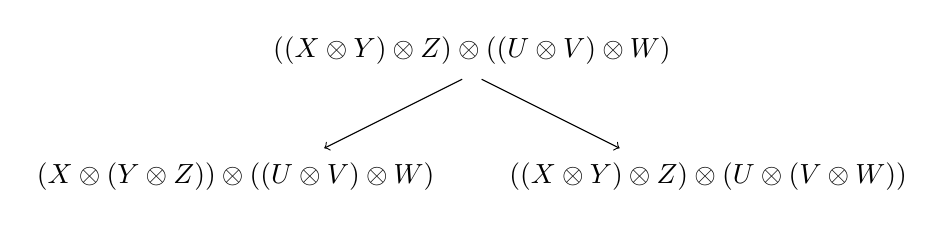
\begin{tikzpicture}
\node (a) at (0,1) {};
\node (b) at (-2,0) {};
\node (c) at (2,0) {};
\draw[->] (a)--(b);
\draw[->] (a)--(c);
\node at (0,1.3) {$((X\otimes Y)\otimes Z)\otimes((U\otimes V)\otimes W) $};
\node at (-3,-0.3) {$(X\otimes (Y\otimes Z))\otimes((U\otimes V)\otimes W) $};
\node at (3,-0.3) {$ ((X\otimes Y)\otimes Z)\otimes(U\otimes (V\otimes W))$};
\end{tikzpicture}
\end{center}

\medskip

\begin{center}
  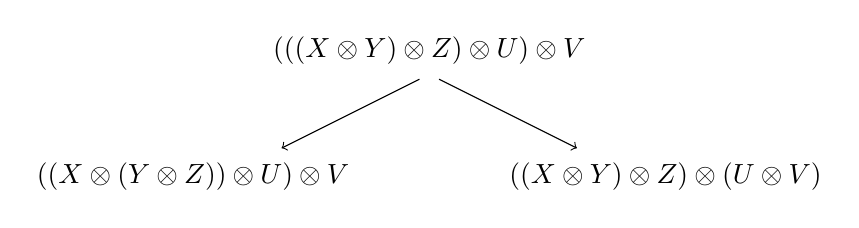
\begin{tikzpicture}
  \node (a) at (0,1) {};
  \node (b) at (-2,0) {};
  \node (c) at (2,0) {};
  \draw[->] (a)--(b);
  \draw[->] (a)--(c);
  \node at (0,1.3) {$(((X\otimes Y)\otimes Z)\otimes U)\otimes V $};
  \node at (-3,-0.3) {$ ((X\otimes (Y\otimes Z))\otimes U)\otimes V$};
  \node at (3,-0.3) {$ ((X\otimes Y)\otimes Z)\otimes (U\otimes V)$};
  \end{tikzpicture}
\end{center}

As we have seen in \cref{non-contextual-2}, this interpretation would not hold anymore if one were to consider the cycle graph instead of the line graph, that is, if one were to identify $X$ and $V$ in the expressions above. 

%%%%%%%%%%%%%%%%%%%%%%%%%%%%%%%%%%%%

\subsubsection{Operahedra}
In the case of operahedra, it turns out that the shape of a $\set{x_1,x_2,x_3}$-face is entirely determined by the relative positions of the edges $x_1,x_2,x_3$ in the underlying  planar tree.  Let us make this more precise.
% Again, one reads constructs directly on operadic trees rather than on their line graph. This leads to a representation of constructs as pairs
%$({\cal S},w)$, where $w$ is a partially parenthesised word ``suiting'' ${\cal S}$. For example, applying the same recipe as in~\cref{Huet-MacLane}, for the operadic tree ${\cal T}$ of~\cref{fig:line-graph}, the construct 
%$z(x(y),u)$ is represented as $({\cal T},(c(bd))(ae)$. We refer to~\cite{CO-categorified}[Section 2.4.3] for details.
Let $S$ be an $X$-face of $\mathbb{L}({\cal T})$, for some  planar tree $\cal T$. Then its shape is given by (the line graph associated to)  the tree ${\cal T}_{\setminus X}$ obtained from  ${\cal T}$  by contracting all edges except the three elements of $X$ (which are edges of ${\cal T}$).  We leave the details to the reader, but note that
this illustrates contextuality: this shape is only determined by ${\cal T}$ and $X$, and does not depend on the position of $X$ in $S$.

Let us also say a word on the actual coherence statement for categorified operads: it relies on a signature and rewrite rules much in the spirit of the Huet--Mac Lane rewriting system (see~\cite{DP15,laplante-anfossiDiagonalOperahedra2022a,CLA1}), that correspond to  constructs of operahedra,  to their equivalent representations as nestings of planar trees (the linear trees of associahedra being a particular case), and to our rewriting systems on the line graphs of planar trees. 

%%%%%%%%%%%%%%%%%%%%%%%%%%%%%%%%%%%%

\subsubsection{Permutahedra and friends}
It seems likely that the family of permutahedra admits a similar categorical coherence theorem. 
The corresponding algebraic structure would be here that of \emph{permutads} \cite{LodayRonco11,Markl19}. 
In the same fashion as associahedra are operahedra associated to linear trees, permutahedra are operahedra associated to $2$-leveled trees \cite[Def.~2.8]{laplante-anfossiDiagonalOperahedra2022a}.
Therefore, one could define categorified permutads by adapting the definition of categorified operads \cite{CLA1} to these trees.

In the case of contextual graph-associahedra, it seems likely that a corresponding coherence theorem could be associated to a certain type of categorified reconnectads \cite{DotsenkoKeilthyLyskov}.
The situation is summarized in \cref{table:contextual-hyper}.

\begin{table}[h!]
	\begin{center}
	\begin{tabular}{c|c|c}
	Family & Algebraic structure & Coherence theorem \\
	\hline
	Simplices & - & - \\
	Cubes & - & - \\
	Associahedra & Monoidal category & \cite{MacLane63} \\
	Permutahedra & Categorified permutads & - \\
	Operahedra & Categorified operads & \cite{DP15,CLA1} \\
	Contextual graph-associahedra & Categorified reconnectads & - \\
	Contextual nestohedra & - & - 
	\end{tabular}
	\end{center}
  \caption{Families of contextual hypergraphs, the categorical structures that they (conjecturally) encode, and their associated coherence theorems.}
  \label{table:contextual-hyper}
\end{table}






